\ifdefined\beamerclass
\else
    \def\beamerclass{beamer}
\fi
\documentclass[\beamerclass]{beamer}

\usepackage{pgfpages}
\mode<handout>{
  % \setbeamercolor{background canvas}{bg=black!20}
  \pgfpagesuselayout{2 on 1}[a4paper,border shrink=5mm]
}

\usepackage{lmodern}
\usepackage{listings}
\usepackage{amsmath}
\usepackage{bm}
\usepackage{textpos} % package for the positioning

\usepackage{pgf, tikz}
\usetikzlibrary{arrows, automata}

\usetheme{Copenhagen}
\hypersetup{pdfstartview={Fit}}
\lstset{basicstyle=\small\ttfamily,breaklines=true}

\usepackage[english]{babel}
\usepackage{algorithm}
\usepackage[noend]{algpseudocode}
\usepackage[utf8x]{inputenc}
\usepackage{graphicx}
\usepackage{hyperref}
%\graphicspath{{./images/}}
\usepackage{tikz}
\usetikzlibrary{shapes.geometric, arrows,chains}
\usepackage{booktabs,makecell,multirow,tabularx}
\usepackage{verbatim}
\renewcommand{\arraystretch}{1.2}
\renewcommand\theadfont{\normalfont\bfseries}
\usepackage{array}
\usepackage{listings}
\lstset{language=Java, showstringspaces=false}
\usepackage[normalem]{ulem}
\usepackage{bm}
\def\layersep{2.5cm}

\usepackage{xcolor}
%\usepackage{subfig}
\setbeamertemplate{caption}{\insertcaption}
\usepackage[caption=false]{subfig}
\usepackage{hyperref}
\usepackage{verbatim}
%\setbeamertemplate{caption}[numbered]%\numberwithin{figure}{section}
% Define block styles
\tikzstyle{decision} = [diamond, draw, fill=blue!20, 
    text width=4.5em, text badly centered, node distance=3cm, inner sep=0pt]
\tikzstyle{block} = [rectangle, draw, fill=blue!20, 
    text width=3em, text centered, rounded corners, minimum height=3em]
\tikzstyle{line} = [draw, -latex']
\tikzstyle{cloud} = [draw, ellipse, fill=red!20, node distance=3cm,
    minimum height=2em]
\tikzset{
  startstop/.style={
    rectangle, 
    rounded corners,
    minimum width=3cm, 
    minimum height=1cm,
    align=center, 
    draw=black, 
    fill=red!30
    },
  process/.style={
    rectangle, 
    minimum width=3cm, 
    minimum height=1cm, 
    align=center, 
    draw=black, 
    fill=blue!30
    },
  decision/.style={
    rectangle, 
    minimum width=3cm, 
    minimum height=1cm, align=center, 
    draw=black, 
    fill=green!30
    },
  arrow/.style={thick,->,>=stealth},
  dec/.style={
    ellipse, 
    align=center, 
    draw=black, 
    fill=green!30
    },
}
\tikzstyle{arrow} = [thick,->,>=stealth]

\tikzset{onslide/.code args={<#1>#2}{%
  \only<#1>{\pgfkeysalso{#2}} % \pgfkeysalso doesn't change the path
}}

\makeatletter
\newenvironment<>{btHighlight}[1][]
{\begin{onlyenv}#2\begingroup\tikzset{bt@Highlight@par/.style={#1}}\begin{lrbox}{\@tempboxa}}
{\end{lrbox}\bt@HL@box[bt@Highlight@par]{\@tempboxa}\endgroup\end{onlyenv}}

\newcommand<>\btHL[1][]{%
  \only#2{\begin{btHighlight}[#1]\bgroup\aftergroup\bt@HL@endenv}%
}
\def\bt@HL@endenv{%
  \end{btHighlight}%   
  \egroup
}
\newcommand{\bt@HL@box}[2][]{%
  \tikz[#1]{%
    \pgfpathrectangle{\pgfpoint{1pt}{0pt}}{\pgfpoint{\wd #2}{\ht #2}}%
    \pgfusepath{use as bounding box}%
    \node[anchor=base west, fill=orange!30,outer sep=0pt,inner xsep=1pt, inner ysep=0pt, rounded corners=3pt, minimum height=\ht\strutbox+1pt,#1]{\raisebox{1pt}{\strut}\strut\usebox{#2}};
  }%
}
\makeatother

\definecolor{darkblue}{RGB}{37,55,97}
\definecolor{mellowyellow}{RGB}{247,206,70}
\definecolor{almostwhite}{RGB}{254,255,255}
\definecolor{merrygreen}{RGB}{79,173,91}
\definecolor{funkyorange}{RGB}{240,154,56}

\addtobeamertemplate{footnote}{\hskip -2em}{}
\newcommand\blfootnote[1]{%
  \begingroup
  \renewcommand\thefootnote{}\footnote{#1}%
  \addtocounter{footnote}{-1}%
  \endgroup
}

\DeclareMathOperator{\softmax}{softmax}
\DeclareMathOperator{\ReLU}{ReLU}


%%%%%%%%%%%%%%%%%%%%%%%%%%%%%%%%%%%%%%%%%%%%%%
% Formatting for title page
\title[Visualisation]{Visualisation}
\author{Ethan Harris}  
\institute[]
{
  Vision, Learning and Control\\
  University of Southampton 
}
\date{}
\subject{Computer Science}
\useoutertheme{infolines}
\setbeamertemplate{headline}{} %remove headline
\setbeamertemplate{navigation symbols}{} %remove navigation symbols

%%%%%%%%%%%%%%%%%%%%%%%%%%%%%%%%%%%%%%%%%%%%%%
\begin{document}

\begin{frame}[plain]
  \begin{tikzpicture}[overlay, remember picture, shift={(current page.south west)},font={\fontfamily{Montserrat-TOsF}\selectfont}]
  \fill [mellowyellow,text=darkblue] (0,0) rectangle (\paperwidth, \paperheight);
  \draw (4,7) node [align=left,text=darkblue] {\Huge \begin{tabular}{l} \textbf{Maximise} \\ \textbf{Activations} \end{tabular}};
  \draw (11,1) node [align=left,text=darkblue] {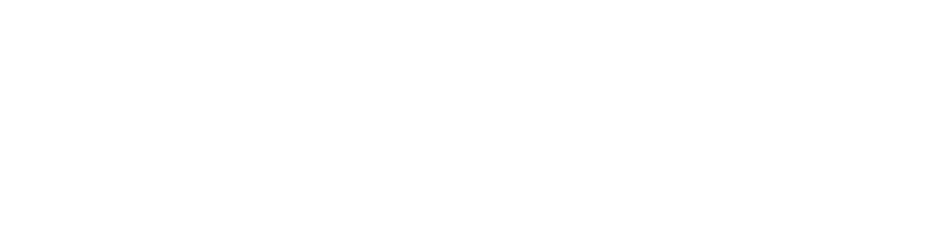
\includegraphics[scale=0.15]{vlc.png}};
  \end{tikzpicture}
\end{frame}


\begin{frame}
  \titlepage%\footnote{Some of the material in this lecture is based on Andrew Ng's lectures on Optimisation} %% \url{https://www.cs.toronto.edu/~tijmen/csc321/slides/lecture_slides_lec6.pdf }} 
\end{frame}

\begin{frame}\frametitle{Overview} 
\begin{itemize}
  \item The Electrophysical and Psychophysical Aspects of Vision
  \item Characterising Single Cells
  \item Feature Visualisation: Monkeys to Machines
  \begin{itemize}
      \item Decorrelation
      \item Reparameterisation
      \item Maximising: Cells, Layers, Predictions
  \end{itemize}
  \item Machines to Monkeys
\end{itemize}
\end{frame}

\begin{frame}\frametitle{Note} 
\begin{itemize}
  \item Feature visualisation article here: \url{https://distill.pub/2017/feature-visualization/}
  \item PyTorch implementations of key algorithms which generated the images can be found here: \url{https://github.com/pytorchbearer/visual}
\end{itemize}
\end{frame}

\begin{frame}\frametitle{The Electrophysical and Psychophysical Aspects of Vision} 
\begin{itemize}
  \item<+-> We want to know the function of the brains input that gives rise to some output
  \item<+-> Inputs - visual stimuli
  \begin{itemize}
      \item<+-> still images, moving stimuli, colour, greyscale, ...
  \end{itemize}
  \item<+-> Outputs - activations
  \begin{itemize}
      \item<+-> single cells, groups of cells, external actions, micro-electrode recordings, fMRI, ...
  \end{itemize}
\end{itemize}
\end{frame}

%%-------------------------------------------------------------%

\begin{frame}
  \frametitle{Characterising Single Cells}
  \begin{itemize}
      \item<+-> Using a micro-electrode recording from a cell, we can plot the \textbf{response curve} to a range of stimuli
      \item<+-> Need to restrict to some controlled stimuli space - colour? edge orientation?
  \end{itemize}
\end{frame}

\begin{frame}
  \frametitle{Case Study: Colour Opponency}
  \begin{itemize}
      \item<+-> Consider the baseline response (or spontaneous rate) of a cell to an empty visual field (i.e. constant grey-level across the retina)
      \item<+-> Now, we change the colour (wavelength) of the visual stimuli and measure the response
  \end{itemize}
\end{frame}

\begin{frame}
  \frametitle{De Valois: Analysis of Response Patterns of LGN Cells}
  \begin{itemize}
      \item<+-> Macaque Lateral Geniculate Nucleus (LGN) cells
  \end{itemize}
  \centering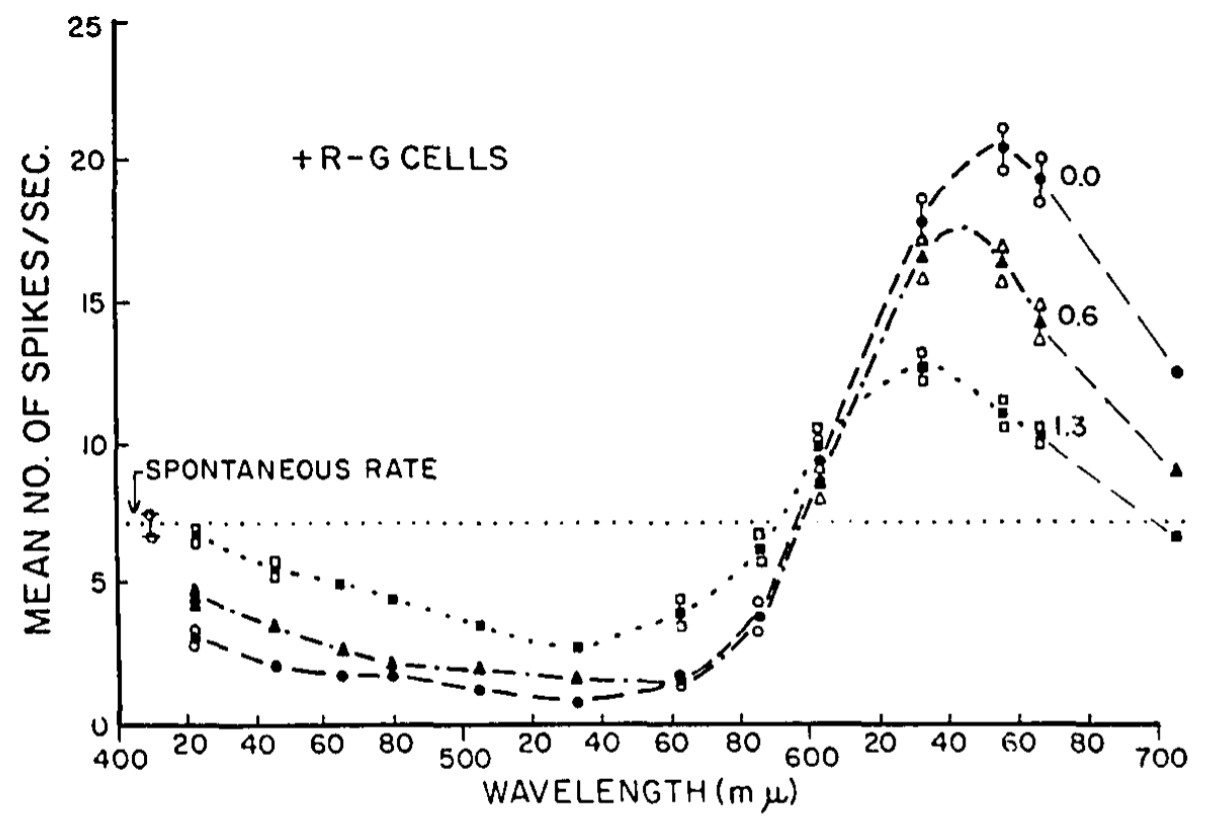
\includegraphics[width=7cm]{devalois.png}
  \begin{itemize}
      \item<+-> Opponent if the curve crosses the line - Non-opponent otherwise
      \item<+-> An analogous form of opponency can be defined - \textbf{spatial} opponency
      \item<+-> Cells which are both spatially opponent and colour opponent are called \textbf{double} opponent
  \end{itemize}
\end{frame}

\begin{frame}{Opponency in Deep Networks}
    \begin{itemize}
        \item<+-> Turns out both spatial and colour opponency happen in deep networks too!
        \item<+-> We measure in \textbf{exactly} the same way as we would in a Monkey - but on a much bigger scale
        \item<+-> More here: \url{https://github.com/ecs-vlc/opponency}
    \end{itemize}
    \centering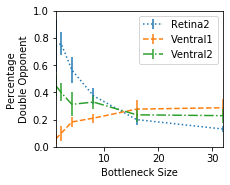
\includegraphics[width=5cm]{double_opponent.png}
\end{frame}

\begin{frame}{Feature Visualisation: Monkeys to Machines}
    \begin{itemize}
        \item<+-> We can also ask the question 'what most excites this cell?' in a deep network
        \item<+-> We've shown a range of stimuli and plotted a response curve as with the monkey
        \item<+-> Can we do something smarter?
        \item<+-> Gradient ascent - use the gradient information we have to `learn' the image which maximises the response of a particular cell or channel
    \end{itemize}
\end{frame}

\begin{frame}{Gradient Ascent}
    \centering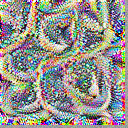
\includegraphics[width=5cm]{plain.png}
    \begin{itemize}
        \item<+-> Inception V3, Layer 6 - Noisy image - not very informative
        \item<+-> Gradient ascent makes an \textbf{uncorrelated} update in a \textbf{correlated} space - hence the crazy colours
    \end{itemize}
\end{frame}

\begin{frame}{Colour Correlation}
    \begin{itemize}
        \item<+-> Compute the RGB correlation statistics from ImageNet
        \item<+-> Correlate the colour channels of the input according to these statistics at each step - now the gradient update is over the \textbf{uncorrelated} parameters
        \item<+-> This type of trick is referred to as \textbf{re-paramterisation} or \textbf{preconditioning}
        \item<+-> The maxima don't change - but the loss surface does - some optima become more likely to be found
    \end{itemize}
\end{frame}

\begin{frame}{Colour Correlation}
    \centering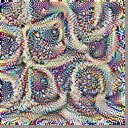
\includegraphics[width=5cm]{correlated.png}
    \begin{itemize}
        \item What can we do about the noise?
    \end{itemize}
\end{frame}

\begin{frame}{Frequency Penalisation}
    \begin{itemize}
        \item<+-> We can construct additional loss functions that penalise high frequencies
        \begin{itemize}
            \item Total variation, blur, L1 loss, ...
        \end{itemize}
        \item<+-> It's better - but we have other ways to improve optimisation procedures
    \end{itemize}
    \centering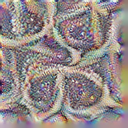
\includegraphics[width=5cm]{penalised.png}
\end{frame}

\begin{frame}{Augmentation}
    \begin{itemize}
        \item<+-> Randomly transform our image before each step
        \item parameters $\to$ correlation $\to$ frequency penalisation $\to$ augmentation $\to$ model
        \item<+-> We know the importance of correlation - what else is correlated in natural images?
    \end{itemize}
    \centering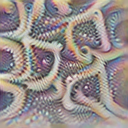
\includegraphics[width=5cm]{augmented.png}
\end{frame}

\begin{frame}{Fourier Space}
    \begin{itemize}
        \item<+-> Space! pixel values are correlated with their neighbours
        \item<+-> But how do we model spatial correlation?
        \item<+-> If a correlation is spatially consistent (i.e. it is constant over the extent of the image) then the Fourier coefficients are \textbf{independent}
        \item<+-> Think of a spatially consistent correlation as a convolution operation
        \item<+-> By the convolution theorem, this is a point-wise multiplication in Fourier space - it treats the coefficients independently
        \item<+-> The Fast Fourier Transform (FFT) is differentiable!
    \end{itemize}
\end{frame}

\begin{frame}{Fourier Space}
    \begin{itemize}
        \item Fourier coefficients $\to$ parameters $\to$ correlation $\to$ augmentation $\to$ model - frequency penalisation is turned off here
        \item That's better!
    \end{itemize}
    \centering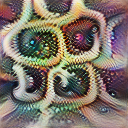
\includegraphics[width=5cm]{fourier.png}
\end{frame}

\begin{frame}{Maximising the Outputs}
    \begin{itemize}
        \item We could also maximise the outputs for a particular class
        \item Here's an Indian Elephant (class 385)
    \end{itemize}
    \centering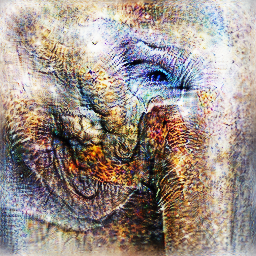
\includegraphics[width=5cm]{elephant.png}
\end{frame}

\begin{frame}{Maximising the Outputs}
    \begin{itemize}
        \item And a Grasshopper (class 311)
    \end{itemize}
    \centering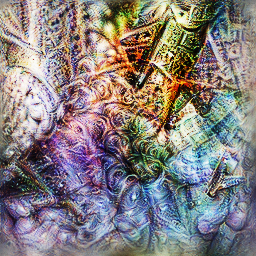
\includegraphics[width=5cm]{grasshopper.png}
\end{frame}

\begin{frame}{Maximising the Outputs}
    \begin{itemize}
        \item Or a Strawberry (class 949)
        \item You get the idea - deep neural networks don't learn about shape!
    \end{itemize}
    \centering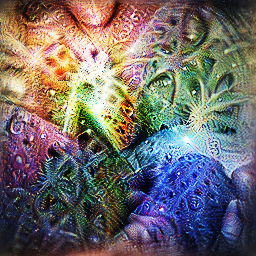
\includegraphics[width=5cm]{strawberry.png}
\end{frame}

\begin{frame}{Maximising the Interestingness}
    \begin{itemize}
        \item<+-> What if we maximise the sum of the squares of the outputs from a whole layer?
        \item<+-> DeepDream! - best results when we start with a real image and gradually increase the scale through training
    \end{itemize}
\end{frame}

\begin{frame}{Mona Lisa}
    \centering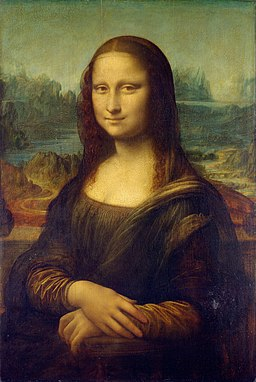
\includegraphics[width=5cm]{mona_lisa.jpg}
\end{frame}

\begin{frame}{Mona Lisa}
    \centering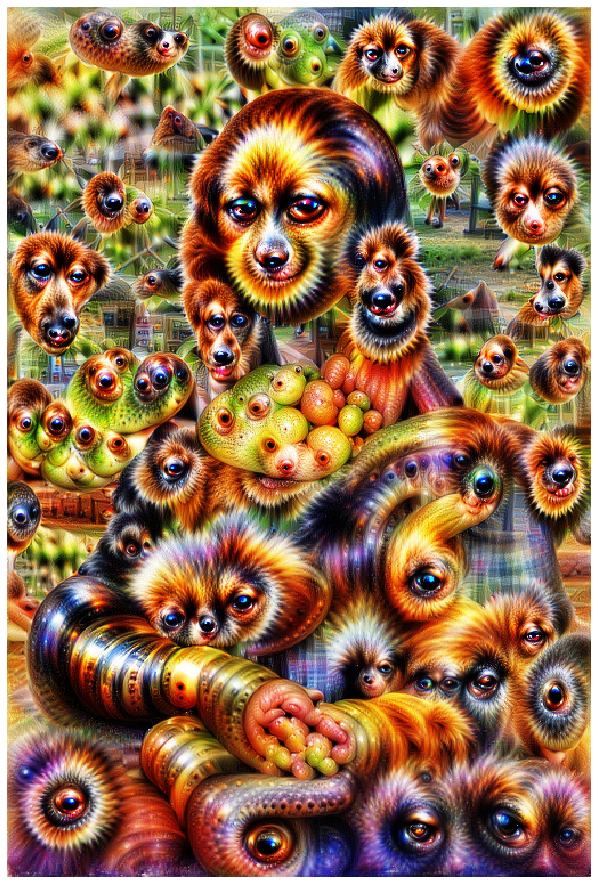
\includegraphics[width=5cm]{mona_lisa_dream.png}
\end{frame}

\begin{frame}{And Back to Monkeys}
    \begin{itemize}
        \item<+-> So we've seen how we can get great visualisations of deep networks
        \item<+-> Much more informative than just looking at single cells
        \item<+-> What's stopping us from doing this in a real brain?
        \item<+-> Nothing! - gradient free optimisers exist - we could use a genetic algorithm
    \end{itemize}
\end{frame}

\begin{frame}{XDREAM}
    \begin{itemize}
        \item Monkey + Genetic Algorithm + Deep Generative Network 
    \end{itemize}
    \centering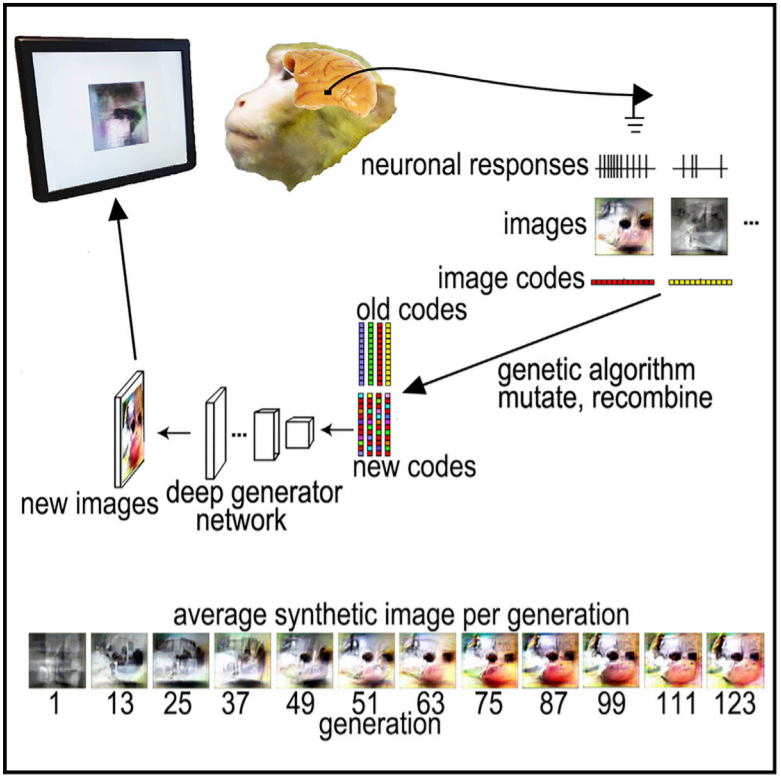
\includegraphics[width=5cm]{xdreamplot.png}
\end{frame}

\begin{frame}{XDREAM}
    \begin{itemize}
        \item Neurons in the Inferior Temporal cortex (AKA the `what' pathway)
    \end{itemize}
    \centering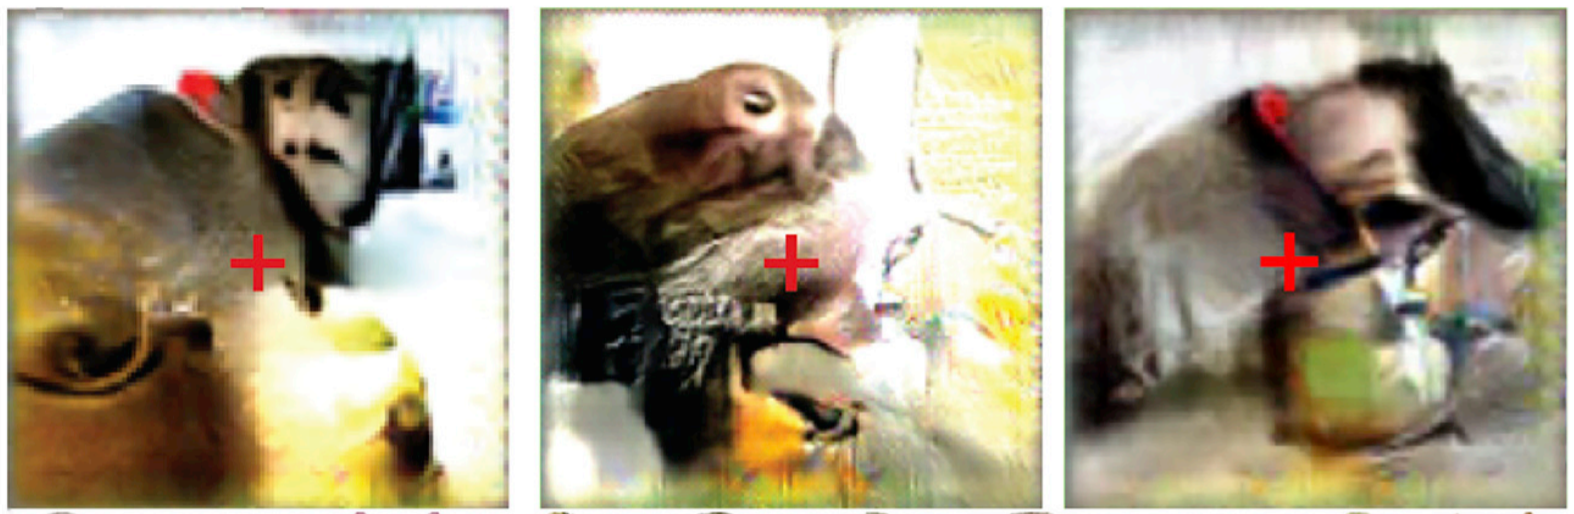
\includegraphics[width=10cm]{xdream.png}
\end{frame}

\begin{frame}{Closing Remarks}
    \begin{itemize}
        \item<+-> Finding the stimuli which maximise the response of single cells has a long history in Neuroscience
        \item<+-> Applying that idea to deep learning we get a way to understand what each `cell' has learned
        \item<+-> But be careful - feature visualisation is more of an art than a science - it isn't a completely solved problem
        \item<+-> Lessons and tools from deep learning can feed back in to Neuroscience, helping us to understand \textbf{much} more complex parts of the brain
        \item<+-> Maybe deep models and brains aren't so different after all!
    \end{itemize}
\end{frame}

%-------------------------------------------------------------%
% \begin{frame}[fragile]\frametitle{Reminder: Gradient Descent}

% \begin{itemize}
%   \item Define total loss as $\mathcal{L} = -\sum_{(\bm x,y) \in \bm D} \ell(g(\bm x,\bm\theta), y)$ for some loss function $\ell$, dataset $\bm D$ and model $g$ with learnable parameters $\bm\theta$.
%   \item Define how many passes over the data to make (each one known as an Epoch)
%   \item Define a learning rate $\eta$
% \end{itemize}

% Gradient Descent updates the parameters $\bm\theta$ by moving them in the direction of the negative gradient with respect to the \textbf{total loss} $\mathcal{L}$ by the learning rate $\eta$ multiplied by the gradient:
% \\[1em]
% \hspace{1cm} \texttt{for each Epoch:}\\
% \hspace{2cm} $\bm\theta \leftarrow \bm\theta - \eta \nabla_{\bm\theta} \mathcal{L}$
% \end{frame}

% %-------------------------------------------------------------%

% \begin{frame}[fragile]\frametitle{Gradient Descent}
% \begin{itemize}
%   \item Gradient Descent has good statistical properties (very low variance)
%   \item But is very data inefficient (particularly when data has many similarities)
%   \item Doesn't scale to effectively infinite data (e.g. with augmentation)
% \end{itemize}
% \end{frame}

% %-------------------------------------------------------------%

% \begin{frame}[fragile]\frametitle{Reminder: Stochastic Gradient Descent}

% \begin{itemize}
%   \item Define loss function $\ell$, dataset $\bm D$ and model $g$ with learnable parameters $\bm\theta$.
%   \item Define how many passes over the data to make (each one known as an Epoch)
%   \item Define a learning rate $\eta$
% \end{itemize}

% Stochastic Gradient Descent updates the parameters $\bm\theta$ by moving them in the direction of the negative gradient with respect to the loss of a \textbf{single item} $\ell$ by the learning rate $\eta$ multiplied by the gradient:
% \\[1em]
% \hspace{1cm} \texttt{for each Epoch:}\\
%   \hspace{2cm} \texttt{for each $(\bm x,y) \in \bm D$:}\\
%     \hspace{3cm} $\bm\theta \leftarrow \bm\theta - \eta \nabla_{\bm\theta} \ell$
% \end{frame}

% %-------------------------------------------------------------%

% \begin{frame}[fragile]\frametitle{Stochastic Gradient Descent}
% \begin{itemize}
%   \item Stochastic Gradient Descent has poor statistical properties (very high variance)
%   \item But is computationally inefficient (poor utilisation of resources - particularly with respect to vectorisation)
% \end{itemize}
% \end{frame}

% %-------------------------------------------------------------%

% \begin{frame}[fragile]\frametitle{Mini-batch Stochastic Gradient Descent}

% \begin{itemize}
%   \item Define a batch size $b$
%   \item Define batch loss as $\mathcal{L}_b = -\sum_{(\bm x,y) \in \bm D_b} \ell(g(\bm x,\bm\theta), y)$ for some loss function $\ell$and model $g$ with learnable parameters $\bm\theta$. $\bm D_b$ is a subset of dataset $\bm D$ of cardinality $b$.
%   \item Define how many passes over the data to make (each one known as an Epoch)
%   \item Define a learning rate $\eta$
% \end{itemize}

% Mini-batch Gradient Descent updates the parameters $\bm\theta$ by moving them in the direction of the negative gradient with respect to the loss of a \textbf{mini-batch} $\bm D_b$, $\mathcal{L}_b$ by the learning rate $\eta$ multiplied by the gradient:
% \\[1em]
% \hspace{1cm}partition the dataset $\bm D$ into an array of subsets of size $b$\\
% \hspace{1cm} \texttt{for each Epoch:}\\
%   \hspace{2cm} \texttt{for each $\bm D_b \in partitioned(\bm D$):}\\
%       \hspace{3cm} $\bm\theta \leftarrow \bm\theta - \eta \nabla_{\bm\theta} \mathcal{L}_b$
% \end{frame}

% %-------------------------------------------------------------%

% \begin{frame}[fragile]\frametitle{Mini-batch Stochastic Gradient Descent}
% \begin{itemize}
%   \item<1-> Mini-batch Stochastic Gradient Descent has reasonable statistical properties (much lower variance than SGD)
%   \item<1-> Allows for computationally efficiency (good utilisation of resources)
%   \item<2-> Ultimately we would normally want to make our batches as big as possible for lower variance gradient estimates, but:
%   \begin{itemize}
%     \item Must still fit in RAM (e.g. on the GPU)
%     \item Must be able to maintain throughput (e.g. pre-processing on the CPU; data transfer time)
%   \end{itemize}
% \end{itemize}
% \end{frame}

% %-------------------------------------------------------------%

% \begin{frame}\frametitle{So, what about the learning rate?}

% \begin{itemize}
% \item<+-> Choice of learning rate is extremely important
% \item<+-> But we have to reason about the `loss landscape'
% \begin{itemize}
%   \item<+-> Most convergence analysis of optimisation algorithms assumes a convex loss landscape
%   \begin{itemize}
%     \item Easy to reason about
%     \item Can be shown that (S)GD will converge to the optimal solution for a variety of learning rates
%     \item Can give insights into potential problems in the non-convex case
%   \end{itemize}
%   \item<+-> Deep Learning is highly non-convex
%   \begin{itemize}
%     \item<+-> Many local minima
%     \item<+-> Plateaus
%     \item<+-> Saddle points
%     \item<+-> Symmetries (permutation, etc)
%     \item<+-> Certainly no single global minima
%   \end{itemize}
% \end{itemize}
% \end{itemize}
% \end{frame}

% %-------------------------------------------------------------%

% \begin{frame}[fragile]\frametitle{*GD in the convex case: failure modes}

% % \begin{itemize}
% % \item If the ellipse is very elongated, the direction of steepest descent is almost perpendicular to the direction towards the minimum
% % \item The gradient vector will have a large component along the short axis of the ellipse and a small component along the long axis of the ellipse.
% % \item This is the opposite of what we want to optimise efficiently
% % \end{itemize}

% 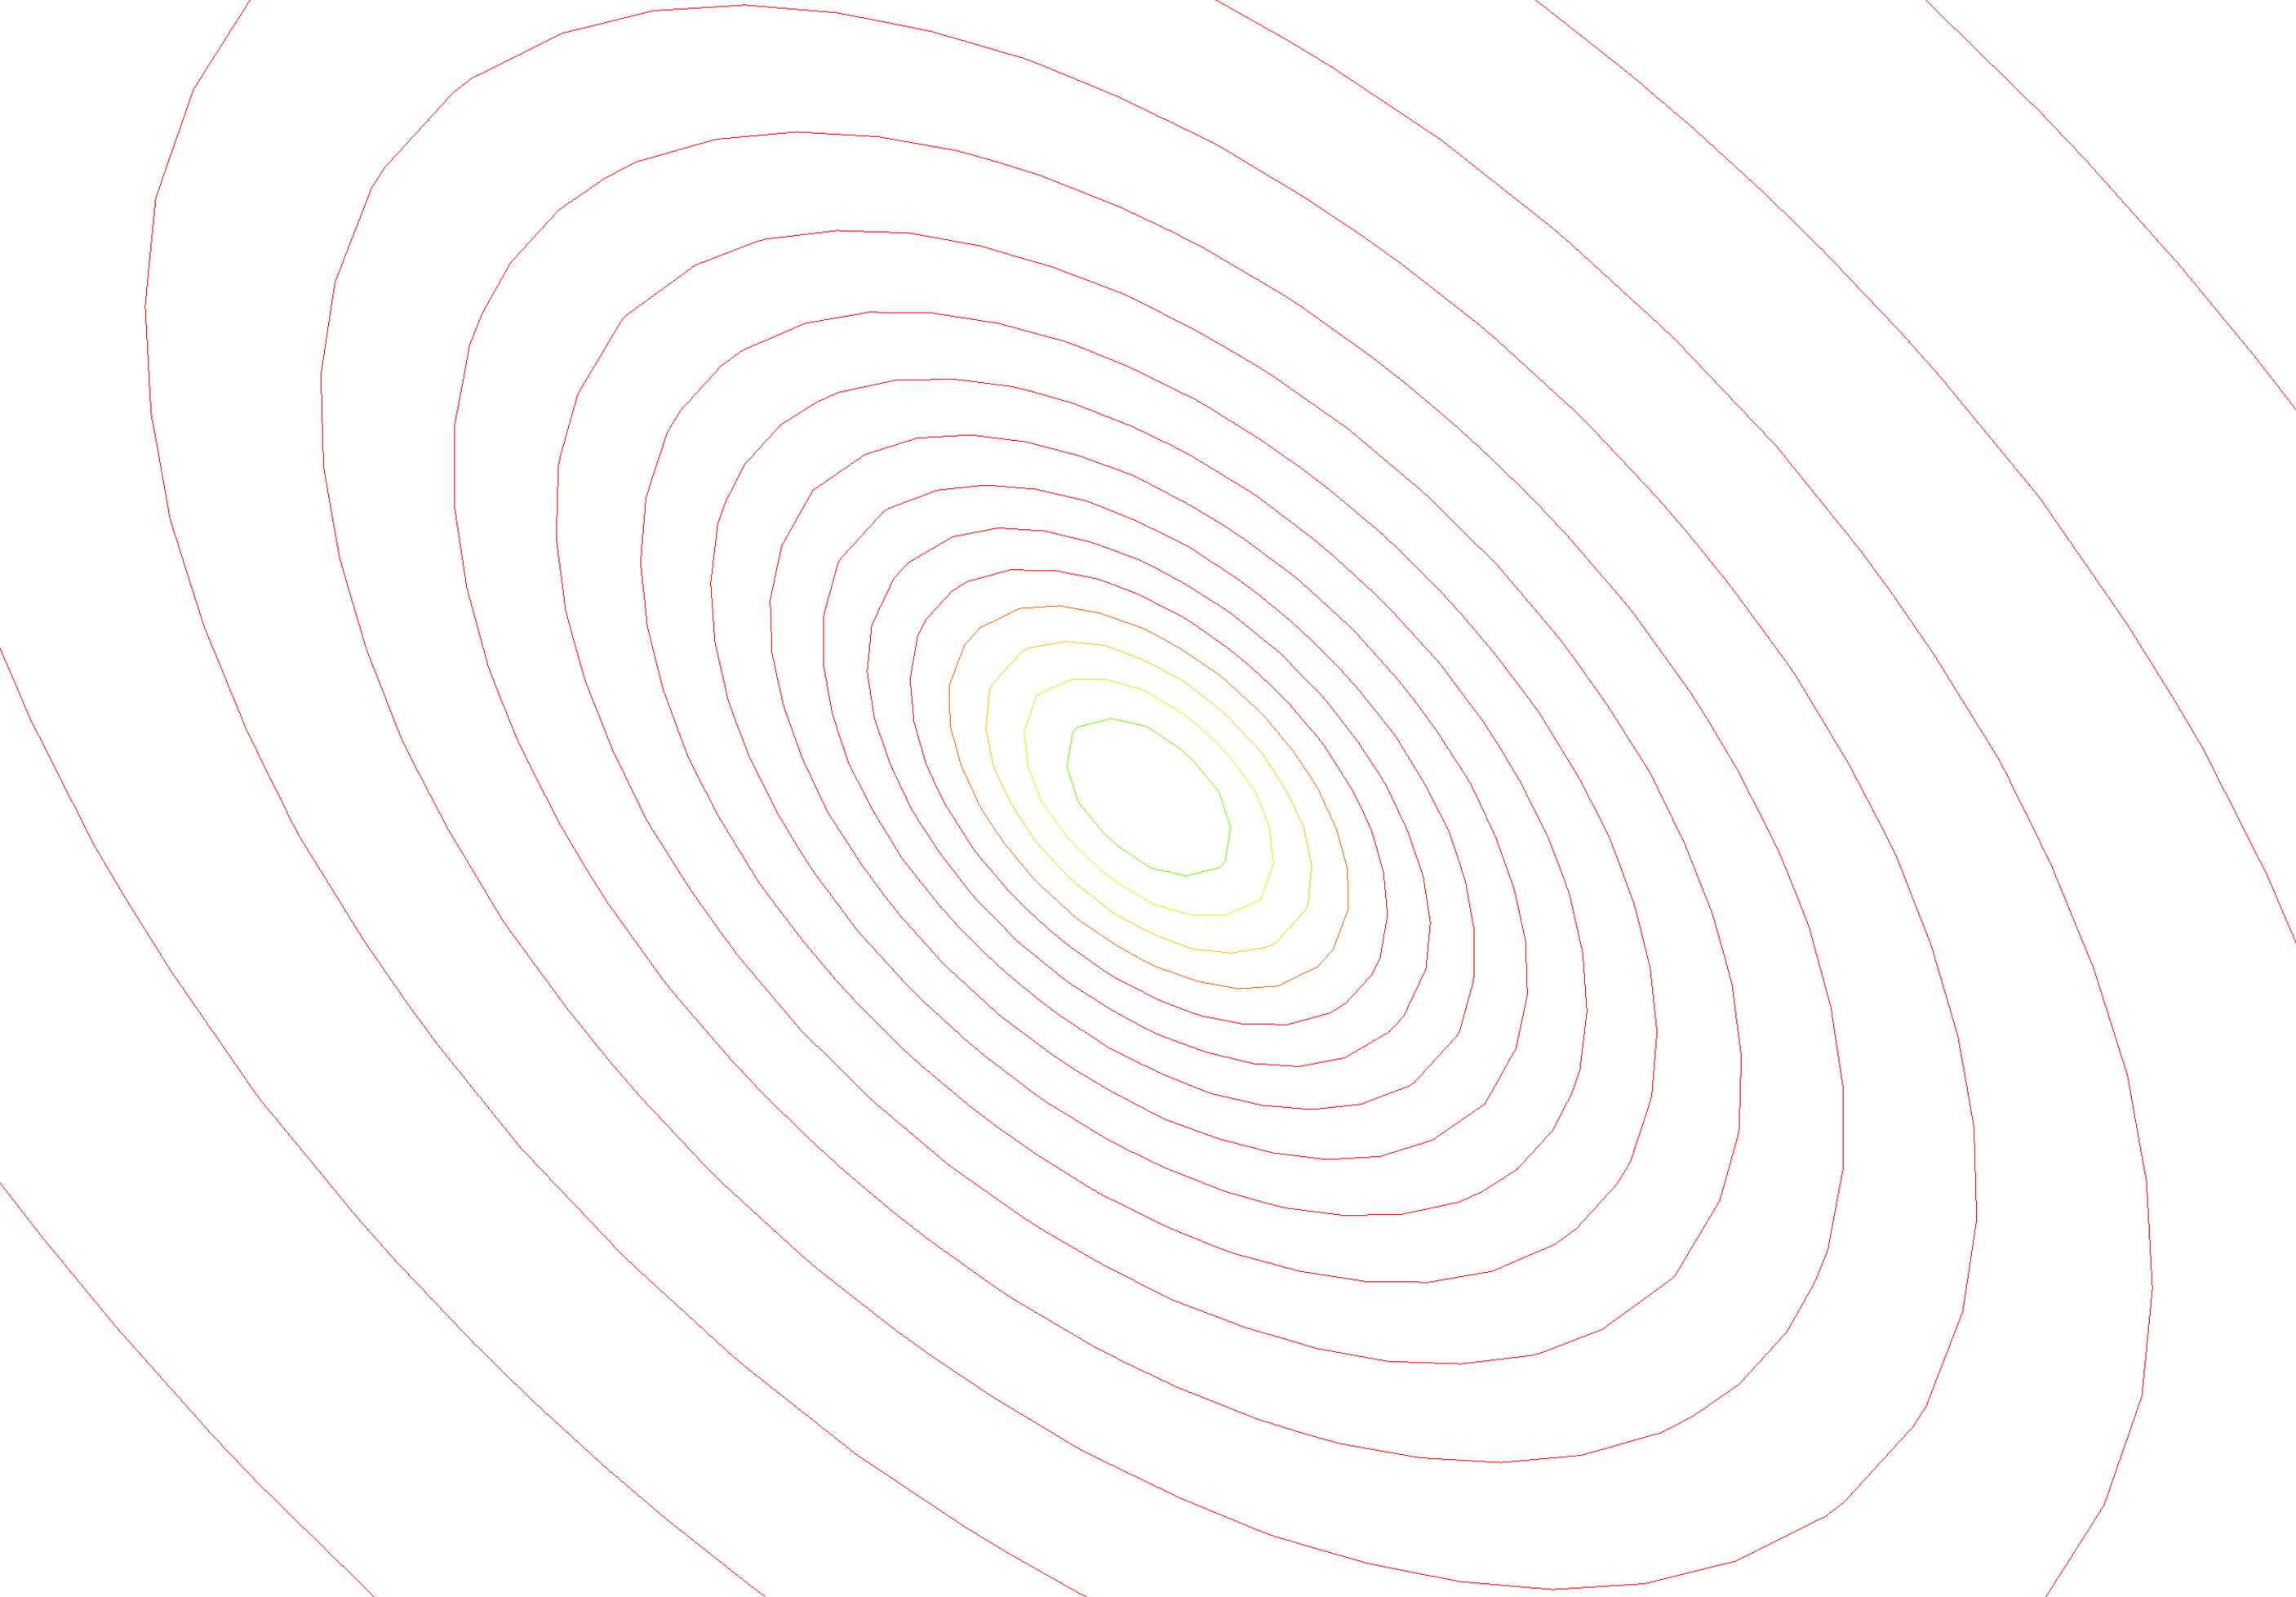
\includegraphics[width=\textwidth]{contours.pdf}

% \end{frame}

% %-------------------------------------------------------------%

% \begin{frame}\frametitle{Accelerated Gradient Methods}

% \begin{itemize}
%   \item<+-> Accelerated gradient methods use a \emph{leaky} average of the gradient, rather than the instantaneous gradient estimate at each time step
%   \item<+-> A physical analogy would be one of the momentum a ball picks up rolling down a hill...
%   \item<+-> As you'll see, this helps address the *GD failure modes, but also helps avoid getting stuck in local minima
% \end{itemize}

% \end{frame}

% %-------------------------------------------------------------%

% \begin{frame}{pause}\frametitle{Momentum I}

% It's common for the `leaky' average (the `velocity', $v_t$) to be a weighted average of the instantaneous gradient $g_t$ and the past velocity\footnote{There are quite a few variants of this; here we're following the PyTorch variant}:

% \begin{equation*}
%   v_t = \beta v_{t-1} + g_t
% \end{equation*}

% where $\beta \in [0,1]$ is the `momentum'.

% \end{frame}
% %-------------------------------------------------------------%


% %\begin{frame}[fragile]\frametitle{ Motivating Momentum}
% %\url{https://www.youtube.com/watch?v=7HZk7kGk5bU&t=172s}
% %\end{frame}
% %-------------------------------------------------------------%

% \begin{frame}[fragile]\frametitle{Momentum II}
% \begin{itemize}
% \item The momentum method allows to accumulate velocity in directions of low curvature that
% persist across multiple iterations
% \item This leads to accelerated progress in low curvature directions compared to gradient descent %\footnote{\url{http://www.cs.utoronto.ca/~ilya/pubs/ilya_sutskever_phd_thesis.pdf}}
% \end{itemize}
% \end{frame}
% %-------------------------------------------------------------%

% \begin{frame}[fragile]\frametitle{MB-SGD with Momentum}

% Learning with momentum on iteration $t$ (batch at $t$ denoted by $b(t)$) is given by:
% \begin{align*}
% \bm v_t & \leftarrow \beta \bm v_{t-1} + \nabla_{\bm\theta} \mathcal{L}_{b(t)} \\
% \bm\theta_t & \leftarrow \bm\theta_{t-1} - \eta \bm v_t
% \end{align*}

% Note $\beta = 0.9$ is a good choice for the momentum parameter.
% \end{frame}
% %-------------------------------------------------------------%

% \begin{frame}\frametitle{SGD with Momentum - potentially better convex convergence}
% 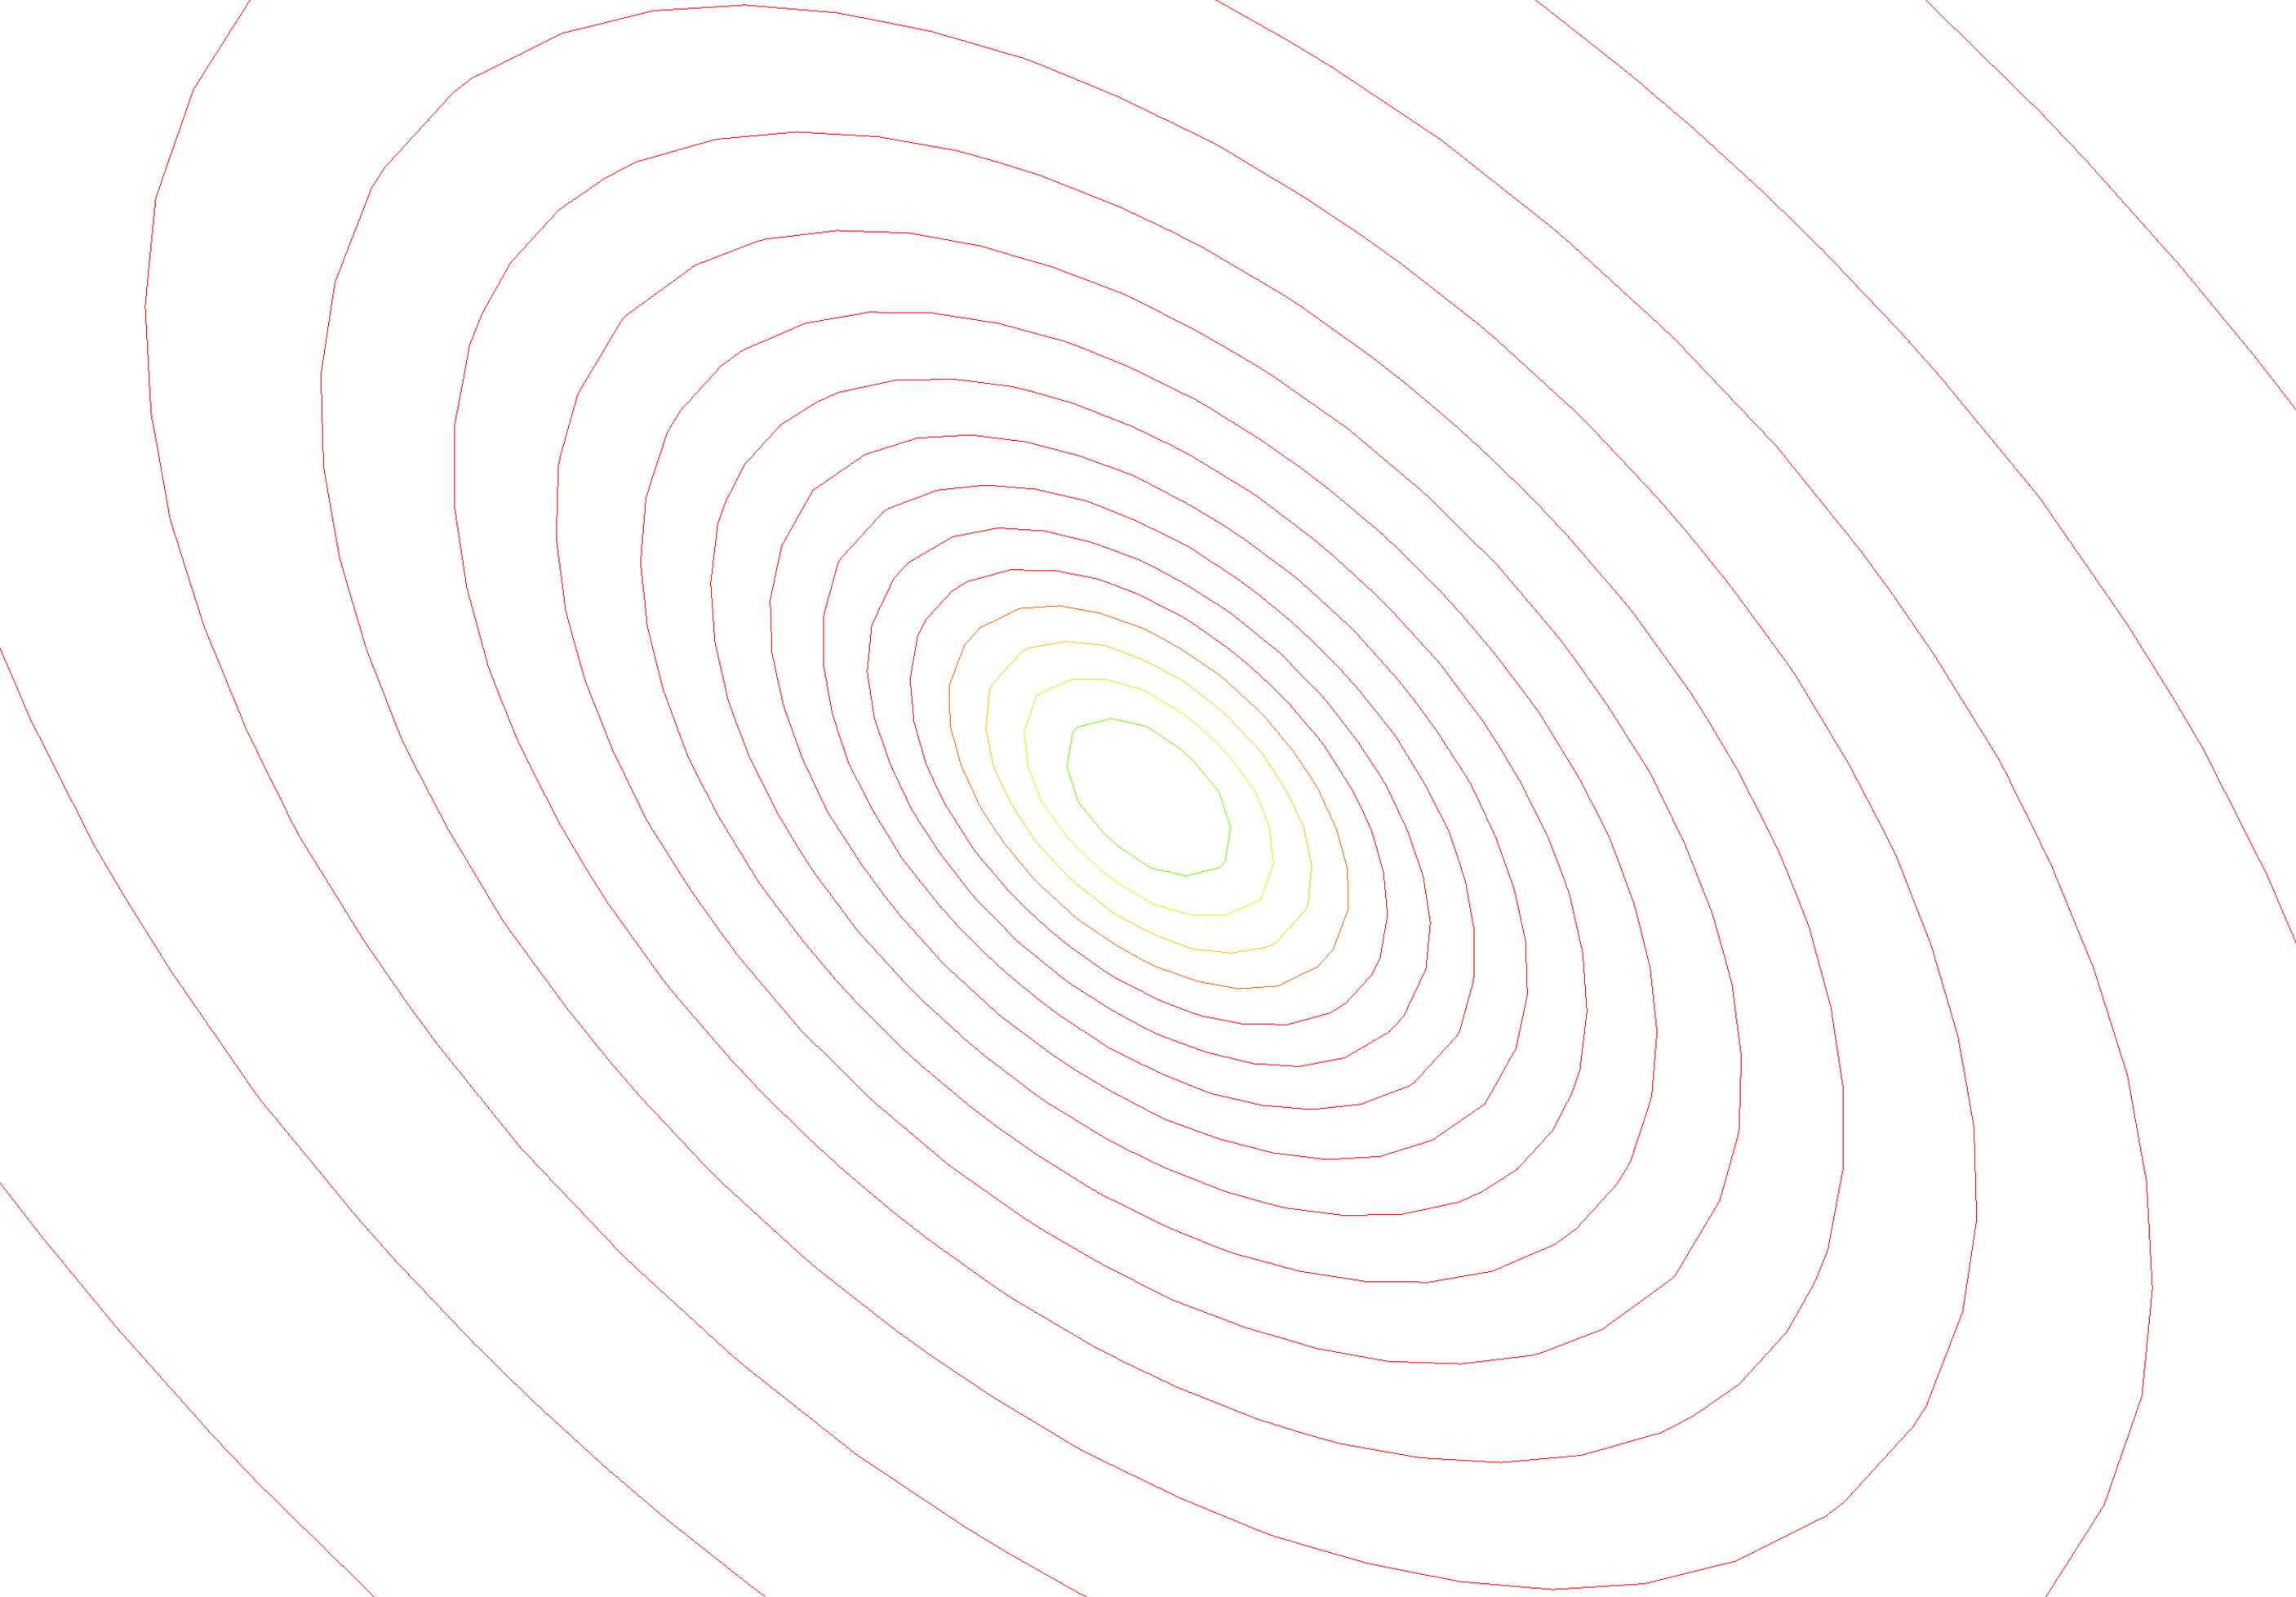
\includegraphics[width=\textwidth]{contours.pdf}
% \end{frame}
% %-------------------------------------------------------------%
% \begin{frame}\frametitle{Learning rate schedules}

% \begin{itemize}
%   \item<+-> In practice you want to decay your learning rate over time
%   \item<+-> Smaller steps will help you get closer to the minima
%   \item<+-> But don't do it to early, else you might get stuck
%   \item<+-> Something of an art form!
%   \begin{itemize}
%     \item `Grad Student Descent' or GDGS (`Gradient Descent by Grad Student`)
%   \end{itemize}
% \end{itemize}

% \end{frame}
% %-------------------------------------------------------------%
% \begin{frame}\frametitle{Reduce LR on plateau}
% \begin{itemize}
%   \item Common Heuristic approach:
%   \begin{itemize}
%     \item if the loss hasn't improved (within some tolerance) for $k$ epochs
%     \item then drop the lr by a factor of 10
%   \end{itemize}
%   \item Remarkably powerful!
% \end{itemize}
% \end{frame}

% %-------------------------------------------------------------%

% \begin{frame}\frametitle{Cyclic learning rates}
% \begin{itemize}
%   \item<+-> Worried about getting stuck in a non-optimal local minima?
%   \item<+-> Cycle the learning rate up and down (possibly annealed), with a different lr on each batch
%   \item<+-> See \url{https://arxiv.org/abs/1506.01186}
% \end{itemize}
% \end{frame}

% %-------------------------------------------------------------%
% \begin{frame}\frametitle{More advanced optimisers}

% \begin{itemize}
%   \item<+-> Adagrad
%   \begin{itemize}
%     \item Decrease learning rate dynamically per weight.
%     \item Squared magnitude of the gradient (2nd moment) used to adjust how quickly progress is made - weights with large gradients are compensated with a smaller learning rate.
%     \item Particularly effective for sparse features.
%   \end{itemize}
%   \item<+-> RMSProp
%   \begin{itemize}
%     \item Modifies Adagrad to decouple learning rate from gradient magnitude scaling
%     \item Incorporates leaky averaging of squared gradient magnitudes
%     \item LR would typically follow a predefined schedule
%   \end{itemize}
%   \item<+-> Adam
%   \begin{itemize}
%     \item Essentially takes all the best ideas from RMSProp and SDG+Momentum
%     \item Bias corrected momentum and second moment estimation
%     \item Shown that it might still diverge (or be non optimal, even in convex settings)...
%     \item LR is still a hyperparameter (you might still schedule)
%   \end{itemize}
% \end{itemize}

% \end{frame}
% %-------------------------------------------------------------%

% \begin{frame}\frametitle{Take-away messages}

% \begin{itemize}
%   \item The loss landscape of a deep network is complex to understand (and is far from convex)
%   \item If you're in a hurry to get results use Adam
%   \item If you have time (or a Grad Student at hand), then use SGD (with momentum) and work on tuning the learning rate
%   \item If you're implementing something from a paper, then follow what they did!
% \end{itemize}

% \end{frame}
%-------------------------------------------------------------%

% \begin{frame}[fragile]\frametitle{RMSProp}
% Learning with RMSProp is given by \vspace{5mm}

% On iteration $t$: \\
% \hspace{3mm} Compute $dW$ on current mini-batch \\
% \begin{eqnarray}
% && S_{dW_t} =  \beta S_{dW_{t-1}} + (1 - \beta) dW_t^2 \\
% && w_t = w_{t-1} - \eta \frac{dW_t}{\sqrt S_{dW_t}} 
% \end{eqnarray}

% \end{frame}
% %-------------------------------------------------------------%


% \begin{frame}{pause}\frametitle{Bias Correction Motivation}

% \begin{itemize}
% \item Let's  assume that $v_0 = 0$ and $\beta = 0.9$ and we're considering exponentially weighted averages \pause
% \item It follows that $v_1 = \beta (0) + (1 - \beta) \theta_1 = 0.1 \hspace{1mm} \theta_1$  \pause
% \item and $v_2 = \beta ( (1 - \beta) \theta_1) + (1-\beta) \theta_2 = 0.0196 \hspace{1mm} \theta_1 + 0.02 \hspace{1mm} \theta_2 $ \pause
% \end{itemize}
% \end{frame}
% %-------------------------------------------------------------%

% \begin{frame}{pause}\frametitle{Bias Correction }

% \begin{itemize}
% \item Add a bias correction term: $\frac{v_t}{1 - \beta^t} $\pause
% \item $t = 1$: $\frac{v_1}{1 - (0.9)^1} = 10 * v_1$ \pause
% \item $t = 2$: $\frac{v_2}{1 - (0.9)^2} = 5.263 * v_2$ \pause
% \item \dots
% \item $t = 10$: $\frac{v_{10}}{1 - (0.9)^{10}} = 1.535 * v_{10}$ 
% \item \dots
% \item $t = 20$: $\frac{v_{20}}{1 - (0.9)^{20}} = 1.138 * v_{20}$ 
% \end{itemize}
% \end{frame}
% %-------------------------------------------------------------%

% \begin{frame}[fragile]\frametitle{ Adam}
% Initialize parameters: $V_{dW} = 0, S_{dW} = 0$ \vspace{3mm}

% On iteration $t$: \\
% \hspace{3mm} Compute $dW_t$ on current mini-batch \\
% \begin{eqnarray}
% && V_{dW} =  \beta_1 V_{dW} + (1 - \beta_1) dW, \hspace{3mm} V_{dW}^{corr} = \frac{ V_{dW}} { (1 - \beta_1^t)}\\ 
% && S_{dW} =  \beta_2 S_{dW} + (1 - \beta_2) dW^2 , \hspace{3mm} S_{dW}^{corr} = \frac{ S_{dW}} { (1 - \beta_2^t)}\\ 
% && w := w - \eta \frac{V_{dW}^{corr}}{\sqrt (S_{dW}^{corr} + \epsilon)}
% \end{eqnarray}

% \end{frame}
%-------------------------------------------------------------%


\end{document}
